\section{Gráficas}

Se grafican los datos de \ref{tab:postiemcono} y la velocidad.

\clearpage
\begin{figure}[h!]
    \centering
    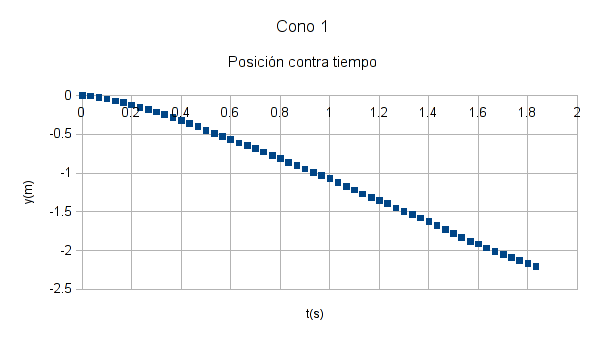
\includegraphics{pos_time1}
    \caption{Gráfica de posición contra tiempo para el cono 1. Se puede 
    observar que a partir de $t$ igual a 0.4 s se alcanza la velocidad
    terminal.}
    \label{fig:posl_cono1}
\end{figure}

\begin{figure}[h!]
    \centering
    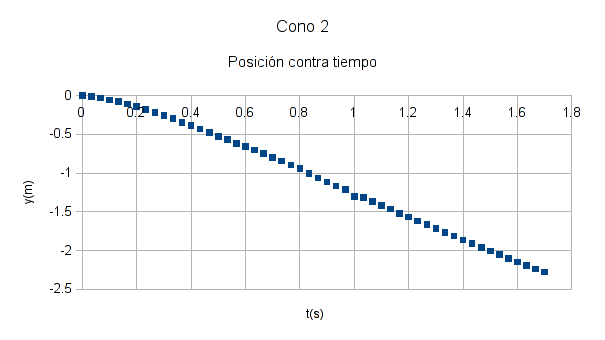
\includegraphics{pos_time2}
    \caption{De nuevo se observa que el cono alcanza su velocidad terminal en
    el instante $t$ igual a 0.3 s.}
    \label{fig:pos1_cono2}
\end{figure}

\begin{figure}[h!]
    \centering
    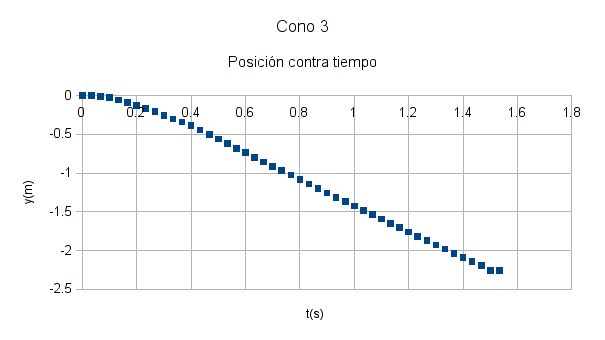
\includegraphics{pos_time3}
    \caption{Gráfica de posición contra tiempo del cono número 3.
    La velocidad terminal es alcanzada en el tiempo 0.25 s.}
    \label{fig:pos1_cono3}
\end{figure}
